\chapter{Bewertung}

Das Ergebnis dieser Arbeit ist ein innovatives, funktionstüchtiges Werkzeug, das in der Lage ist dem
Nutzer bei der Arbeit mit Beweisdokumenten eine sinnvolle und produktive Unterstützung zu gewähren.
Als Maßstab für die Einordnung der Ergebnisse bietet sich ein Vergleich mit dem bisherigen Ansatz
Isabelle/jEdit an. 

Dabei ist allerdings zu beachten, dass es sich bei diesem Projekt auch um eine Machbarkeitsstudie
für die Umsetzung einer webbasierten IDE handelt, da es nicht möglich ist eine sogenannte
\textit{full featured} IDE im Rahmen einer Diplomarbeit zu entwickeln und dabei zusätzlich die
zahlreichen neuen Aspekte im Zusammenhang mit der Kommunikation einer speziellen Webanwendung zu
beachten.

\section{Performanz}

Da die selbe Bibliothek (Isabelle/Scala) wie in der jEdit Version zu Grunde liegt, gibt es keine
Unterschiede in der Geschwindigkeit des Beweisers selbst. Bei der lokalen Ausführung auf einem
Rechner mit Server und Browser ist zu erwarten, dass es durch die Kommunikation über serialisierte
Nachrichten und deren Umrechnung zu leichten Geschwindigkeitseinbußen gegenüber Isabelle/jEdit
kommt. Die Performanz auf diese Weise zu vergleichen is jedoch nicht sinnvoll, da in einem
gewöhnlichen Szenario der Server auf einem zentralen Rechner ausgeführt wird, der über die nötigen
Ressourcen verfügt, um die Isabelle Plattform tragen zu können. Der Zugriff geschieht dann über
mehrere Clients, die keine besonders hohen Ansprüche erfüllen müssen. Hier liegt ein Vorteil
gegenüber der jEdit Implementierung. Mit \textit{clide} ist es theoretisch möglich, einen
Theorembeweiser von einem Netbook oder einem Tablet PC aus zu verwenden.

\section{Funktionalität}

Die geforderten Funktionen konnten alle implementiert werden. Es existieren vielfältige
Möglichkeiten für den Nutzer.

Ein Nachteil gegenüber dem Proof General ist die fehlende Möglichkeit der \textbf{semantischen
Suche} in Isabelle Quellen. Diese Funktionalität wird von der Isabelle Plattform bereit gestellt und
ist bis jetzt leider von der Isabelle/Scala Schnittstelle noch nicht unterstützt (und daher auch in
Isabelle/jEdit nicht vorhanden).

Darüber hinaus fehlt natürlich die Infrastruktur an Plugins welche für jEdit existiert, da es sich
bei der Anwendung notwendiger Weise um eine Neuentwicklung handelt. Das macht es natürlich mühsamer
zusätzliche Funktionalität wie Versionsverwaltungssystem oder andere Erweiterungen, zu integrieren,
da diese dann speziell für diese neue Plattform entwickelt werden müssen.

Eine große Zahl von Funktionen ist nur über Tastenkürzel verfügbar, jedoch nicht über Mausaktionen,
diese Nachzurüsten ist eher Fleißarbeit, da die Infrastruktur für Kommandos in der Sidebar bereits
fertiggestellt wurde. Dieser Umstand betrifft damit eher die Usability in
Abschnitt\,\ref{sec:usability}.

\section{Zuverlässigkeit}

Da die Browseranwendung zwingend in \acr{js}, also einer dynamischen Sprache entwickelt werden
musste ist es schwieriger, Fehler zu entdecken, da Typfehler in sprachen mit dynamischer Typisierung
logischerweise nicht existieren und der Compiler so keine große Hilfe bei der Fehlerfindung
darstellt. Während der Entwicklung wurden sogenannte \textit{cross checks} im Code geführt (Welche
nun auskommentiert sind (Siehe z.B. \texttt{isabelle.coffee})) um die Datenkonsistenz regelmäßig zu
überprüfen. Das reicht aber natürlich nicht aus um die Fehlerfreiheit zu garantieren und da darüber
hinaus das systematische Testen von Benutzeroberflächen immer ein Problem darstellt, kann nicht
ausgeschlossen werden, dass sich noch Fehler in der Benutzerschnittstelle befinden.

Serverseitig mussten vor allem der \texttt{LineBuffer} und das \texttt{RemoteDocumentModel} getestet
werden. Hierfür wurde zum einen eine zuschaltbare Visualisierung der Serverseitigen Daten
implementiert sowie einige in ScalaTest implementierte Testfälle (\texttt{/test/scala/...}). Die
meiste andere Funktionalität stammt aus Isabelle/Scala bzw. Play und wurde nur verknüpft.

\section{Benutzbarkeit}
\label{sec:usability}

Da es sich um eine Benutzerschnittstelle handelt ist Usability ein wichtiges Thema. Da es sich hier
um eine Machbarkeitsstudie handelt, wurden einige Aspekte der Usability zunächst hinten angestellt.
Insbesondere auch die Barrierefreiheit, da diese in einer \textit{single-page}-HTML-Anwendung
bislang schwer zu erreichen ist, nicht zuletzt auch weil viele unkonventionelle ELemente verwendet
werden mussten. Anstelle von ausgiebigen Usability Tests wurde die Anwendung einigen Probanden
(Kommilitonen) zur Benutzung vorgelegt, und deren Verhalten beobachtet. Dabei wurden einige Lücken
gewahr, die noch geschlossen werden konnten. So wurden beispielsweise nach den Tests die meisten
Kommandos auf Standard Tastenkombinationen gelegt oder eigene modale Dialoge anstelle der Browser-
Dialoge eingeführt.

Isabelle/jEdit hat hier natürlich den Vorteil, dass es in einer ausgereiften Umgebung (jEdit) lebt,
die über einige hundert Personenjahre Entwicklungszeit entstanden ist und damit vielfältiger ist.

Die Grundlagen für eine benutzerfreundliche Anwendung wurden aber dennoch geschaffen. Insbesondere
wurde von Anfang an viel Wert auf die \texttt{User Experience} gelegt. In den oben erwähnten Tests
wurde diese häufig als gut gelungen bewertet und es konnte beobachtet werden, dass die Probanden
Spaß an der Nutzung der Anwendung hatten, selbst bei denen, die das eigentliche Thema des
Theorembeweisens nicht interessierte. Das ist eine gute wichtige Voraussetzung für den erfolgreichen
Einsatz in der Lehre, da für das Lernverhalten Emotionen eine wichtige Rolle spielen
\cite{emotionaldesign}.

\section{Visualisierung}

\begin{figure}[ht]
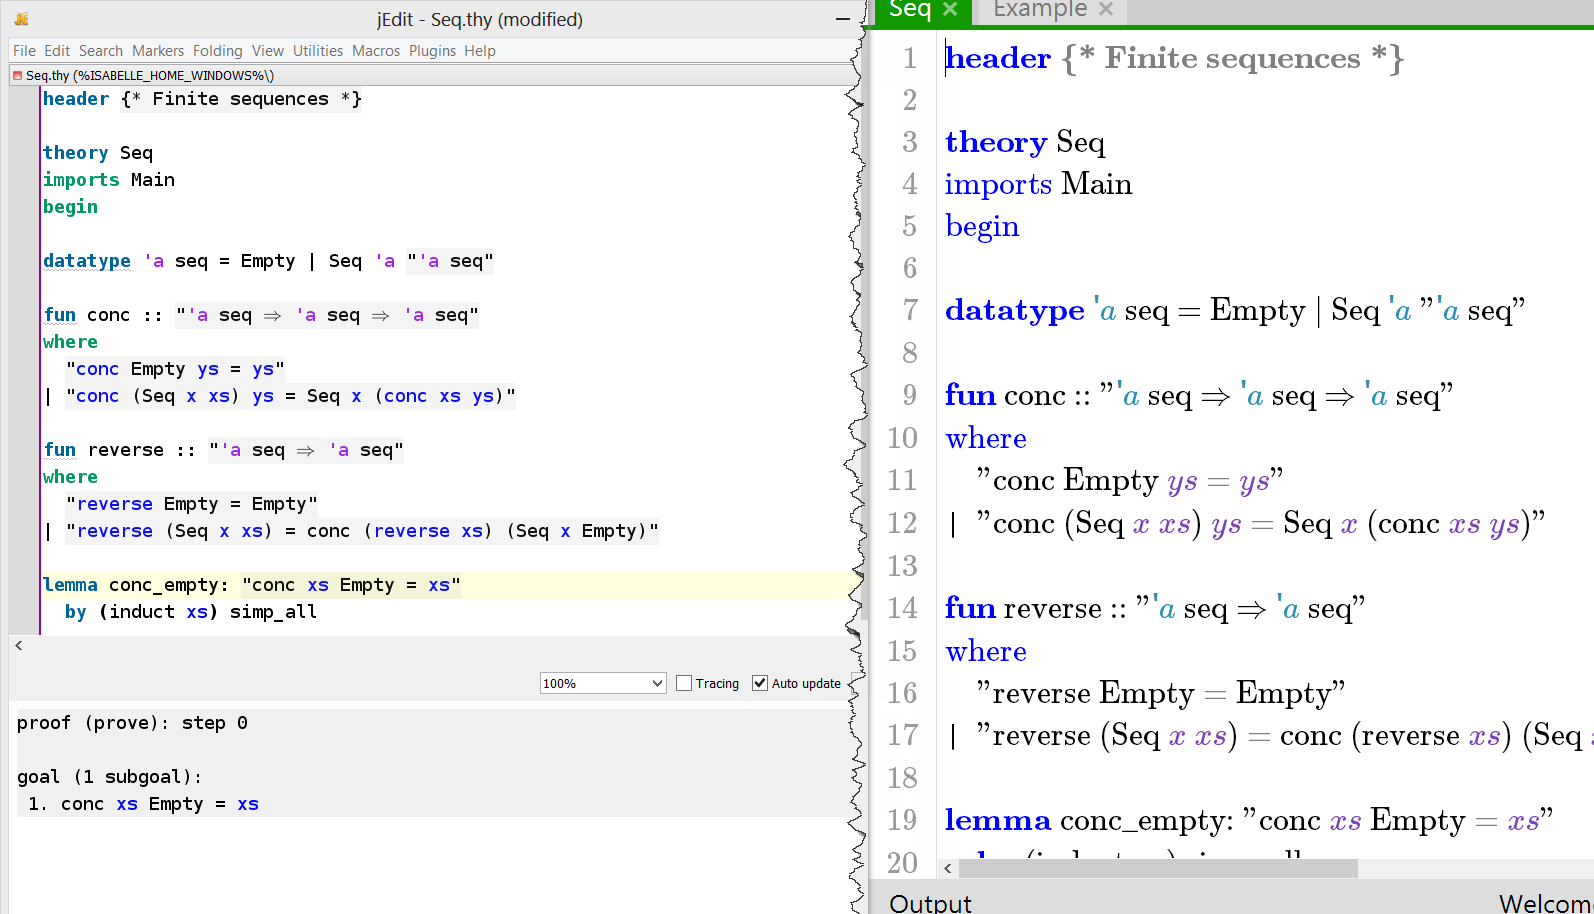
\includegraphics[width=\linewidth]{images/jedit}
  \caption{jEdit vs. clide}
  \label{fig:jedit}
\end{figure}

Hier ist eine klare Verbesserung gegenüber Isabelle/jEdit zu erkennen. Während Isabelle/jEdit sich
am festen Textraster, welches in jEdit vorgegeben ist, orientieren musste und nur geringe
Abweichungen implementieren konnte, ähnelt die Darstellung in der Bearbeitung bei der Webanwendung
schon sehr stark der endgültigen Darstellung in veröffentlichten \LaTeX-Dokumenten (Siehe
Abbildung\,\ref{fig:jedit})

Darüber hinaus ist die Integration der Beweiser-Ausgaben flexibler gestaltet und es ist auch möglich
diese teilweise oder vollständig \textit{inline} anzuzeigen.

\section{Übertragbarkeit}

\textit{clide} ist auch deswegen so interessant, weil es eine ganz neue Form der Veröffentlichungen
ermöglicht. Durch die gute Visualisierung ist es denkbar, Dokumente direkt mit anderen über die
Webanwendung zu teilen. Diese Visualisierung könnte in Zukunft auch als statische \textit{read-
only}-Variante zur Verfügung gestellt werden. 

Die Webanwendung kann als Grundlage für die Integration weiterer Sprachen im Zusammenhang mit
Theorembeweisen genutzt werden. Für die Lehre wäre es denkbar Aufgaben direkt online zu stellen
und lösen zu lassen. Während Isabelle/jEdit auf einem lokalen Rechner \glqq gefangen\grqq ist,
können hier ganz neue Optionen der Integration gewählt werden.
